%
% LaTeX report template 
%
\documentclass[a4paper,10pt]{article}
\usepackage[final]{graphicx}
\usepackage[english]{babel}
\usepackage[latin1]{inputenc}
\usepackage{comment}
\usepackage{subfigure}
\usepackage[section]{placeins}
\usepackage{float}


%
\begin{document}
%
   \title{Team Cherry Tomato Design Overview}

   \author{Joseph Miller 504744848 \\ Jorge Hurtado 704595625 \\ Xilai Zhang 804796478 \\ Patrick Chau 404793486
 \\ Lab 1B}
          
   \date{}

   \maketitle
   
   \tableofcontents
 
  \newpage
   
\section{Introduction}
This report provides an overview of team Cherry Tomato's design for a large-scale display system capable of displaying various letters across graduation caps fitted with LEDs. We outline the requirements of our project and cover the motivation behind our design choices, as well as our techniques of implementing them. Additionally, we review the complications we faced throughout the quarter and how we managed to overcome them. 
\begin{itemize}
	\item Allow for 30-80 participants.
	\item Account for the lack of signal in Pauley Pavilion.
	\item Account for excess amount of noise with radio and audio communication.
	\item Noticeable lighting effects within the bright environment of graduation.
\end{itemize}

\section{Basic Design}
In an effort to meet all the requirements while keeping a relatively low cost, we came up with the following design. Our system consists of client Raspberry Pi Zero W's attached to graduation caps, a hardware token powered by a Raspberry Pi Zero W, and a server running on a Raspberry Pi 4. Each client will be wired to an LED matrix which acts as the display on the top of student's graduation caps. The cap will also hold a button as a means for requesting a position from the server, which will be derived from the hardware token. Our plan of action for the day of graduation will be to pass our token prior to the commencement of the ceremony amongst the students. The token must be incremented by the students as it is passed along as a method of inputting their own position. Each student will press a button to increment the column in the row they are currently in. If they are given the token from someone behind them, they will increment the row they are in instead. Once the token is set to the correct value, which will be displayed by the 7-segment display on the token, the participant will press the button on their cap to initiate a connection to the server. This will allow participants a chance to sync into our server and provide their location info. The 7-segment display additionally serves to display messages regarding whether the hardware is connected and if the pairing is a success. Once the connection succeeds, the token can continue being passed along. Our server allows clients to join the system at any point in time as well as allow for reconnection and recognition of the same client, restoring their prior location and bypassing the need for manually inputting their position again. We broke up the work into four main components, each to be lead by one team member: server (Xilai), client (Jorge), hardware token (Joey), and communications (Patrick).

\begin{figure}[H]
  \centering
      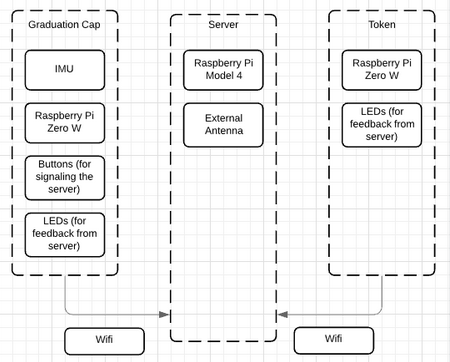
\includegraphics[width=0.8\textwidth]{Assets/overview.png}
  \caption{Diagram outlining the overall design for the project. It displays how the individual components communicate together and what physical hardware is needed to implement each device.}
\end{figure}

\section{Client (Jorge)}
For the first portion of this lab I found that most of my time was spent trying to familiarize myself with the Raspberry Pi interface and available components for the project. Once separated into our groups I was designated to take care of the client. Unfortunately, due to hardware complications our goals for our client were modified throughout the quarter. Our physical outputs were abstracted to print statements which will be replaced once we build our prototype. 

    I overtook developing the code that would parse out the MAC address of clients added to our system. We opted to use MAC addresses as identifiers for our clients because we realized IP addresses might change. Doing so allowed us to retain the positions of all clients that have joined our server incase they reconnected without the possibility of misidentifying a client. After, verifying my code did parse out the address I setup a practice server client connection. I managed to successfully send my Raspberry Pi's MAC address to my laptop. Upon meeting up with our group, we ended up implementing my function into a client designed for Xilai's server. A snippet of the function code is provided below for reference.

\begin{figure}[H]
  \centering
      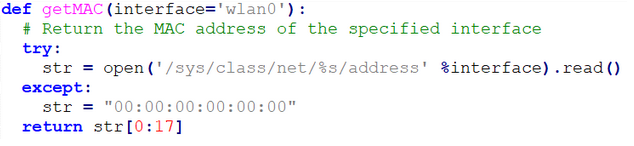
\includegraphics[width=0.8\textwidth]{Assets/MAC_ADDR.png}
  \caption{Code to obtain MAC Address on Raspberry Pi.}
\end{figure}

Additionally, I began developing code for g accelerator and a compass function that would use the data collected from Patrick's log to distinguish whether the participant was standing or walking as part of our standalone lighting function. Additionally, Patrick and I managed to do some test runs so we could acquire data from the IMU and begin looking for identifiers for distinguishing whether individuals are walking or sitting. Unfortunately, I did not finish implementing this as we began to focus on meeting the final requirements.

    In the final weeks of the quarter, I worked diligently with Patrick to develop code that would allow our clients to reconnect to our server if they were to lose connection after pairing. We developed a function that would continuously attempt to reconnect once losing connection after pairing. While doing so we found that a simple call to connect would not suffice and we had to create a whole new connection to rejoin the system.  In order to also ensure we saved the location information of each client we had to go back and modify Xilai's server code as well. Getting this function to work correctly ended up taking more time than initially expected. We still have to go back so that we can handle more exceptions in order to ensure our server doesn't crash during graduation.

\section{Server (Xilai)}
Our design starts with a definition of the client class:
\begin{figure}[H]
  \centering
      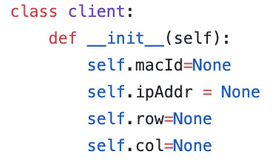
\includegraphics[width=0.3\textwidth]{Assets/client_class.png}
\end{figure}

This client class is expected to store the client-specific information for each Raspberry Pi that establishes connection with the server. Currently we have the MAC Address which is unique for each client, the optional IP address, and the row and column information to store the physical location of the client, namely, the Raspberry Pi Zero W's.

\begin{figure}[H]
  \centering
      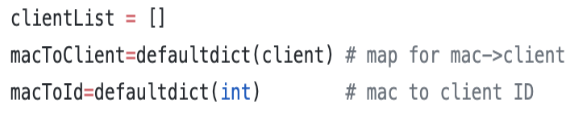
\includegraphics[width=\textwidth]{Assets/client_list.png}
\end{figure}

Here is a glance of data structures we are using for the project. The clientList stores all the clients that have connected to the server. Based on this list, we can later do sorting to generate patterns. The macToClient is dictionary that maps the mac ID of the client to the Client class. In this way, as long as we know the MAC Address, we can retrieve all the other attributes of the client. The macToId maps the MAC Address to a unique client ID. 

\begin{figure}[H]
  \centering
      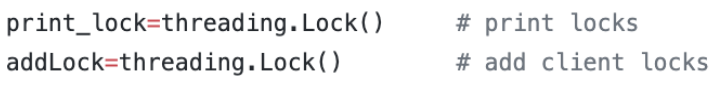
\includegraphics[width=\textwidth]{Assets/locks.png}
\end{figure}

Since we have multiple clients that are trying to communicate with the server and a shared set of structures, we need locks to prevent race conditions from happening. In this project we generate two types of locks. One of them is the print lock. This lock is for situations when we need to log information for debugging purposes. Another lock is the addLock. This lock is the overall lock on the whole set of shared structure. Whenever we wish to make changes on the shared set of data, we need to acquire this lock first.

\begin{figure}[H]
  \centering
      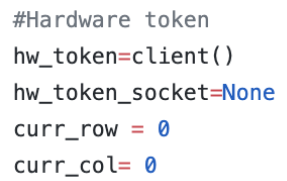
\includegraphics[width=0.3\textwidth]{Assets/token_python.png}
\end{figure}

We treated the hardware token as a client class. We also store the socket id that we have established when the hardware token talks to the server. This allows for us to deliver messages to the hardware token when any individual client thread is successfully added to the server.

\begin{figure}[H]
  \centering
      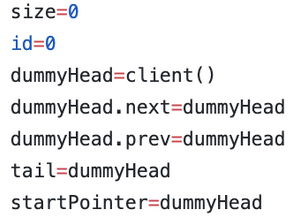
\includegraphics[width=0.3\textwidth]{Assets/snake_params.png}
\end{figure}

Our design supports two functions. One of them is to generate a pattern similar to the game snake where a snake loops around the caps and grows larger, the other is to display characters such as UCLA. To generate the snake pattern, we used a linked list structure. If we follow the linked list starting at startPointer, we would be able to get a consecutive segment of client objects to generate the snake pattern.

\begin{figure}[H]
  \centering
      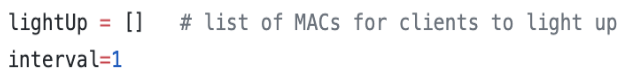
\includegraphics[width=\textwidth]{Assets/light_up.png}
\end{figure}

The global array lightUp stores the client objects that we want to be lit up. During each iteration, the server will scan through all the client objects and update them. The interval variable dictates the length of the snake. Alternative algorithms will eventually be used to determine which caps would be the best to light with a particular pattern and this array will allow for an easy way to signal to every cap when their turn to be lit has arrived.

\begin{figure}[H]
  \centering
      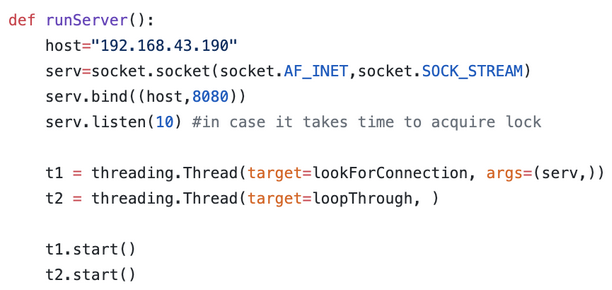
\includegraphics[width=\textwidth]{Assets/run_server.png}
\end{figure}

We will begin our server with two threads, one of them goes to the function lookForConnection, which checks whether there are clients that want to establish a connection with the server. The other thread goes to the function loopThrough, which updates information in the lightUp array to indicate whether a specific client class should be lit up. 

\begin{figure}[H]
  \centering
      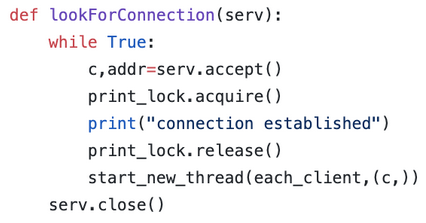
\includegraphics[width=0.9\textwidth]{Assets/look.png}
\end{figure}

In the lookForConnection function, we further split the program into multiple threads, namely, one thread for each connected client. Each connected client will be directed to the function each\textunderscore client, which creates a unique thread for said client. We pass the client socket id to the each\textunderscore client function as well. Along the way, we acquire print lock to log information during the process. 

\subsection{EachClient Function}

\begin{figure}[H]
  \centering
      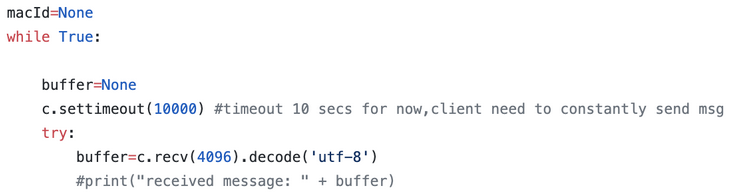
\includegraphics[width=\textwidth]{Assets/timeout.png}
\end{figure}

We start with an empty macId for the thread. Since variables in each thread are defined locally, we can check the status of the current thread by checking the macId variable. If the macId is set, it means we have processed this thread before. If not, the thread is yet to be initialized. In a try loop, we check for response from the client. If we haven't heard back from the client for more than 10 seconds, we assume the client is no longer connected to the server.

\begin{figure}[H]
  \centering
      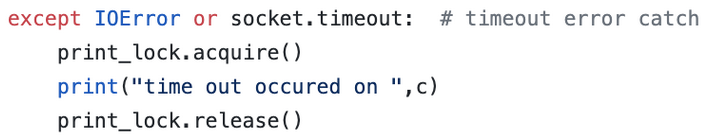
\includegraphics[width=\textwidth]{Assets/except.png}
\end{figure}

\begin{figure}[H]
  \centering
      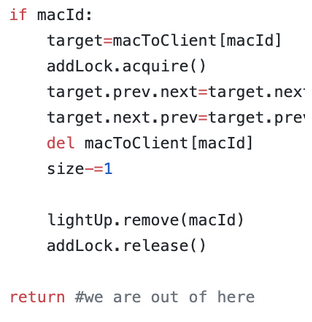
\includegraphics[width=0.5\textwidth]{Assets/if_mac.png}
\end{figure}

In the event of a timeout, we log the timeout message and close the connection. We remove the information of the timed out client from our data structure. Along the way, we will have to acquire the add Lock. 
\pagebreak
\begin{figure}[H]
  \centering
      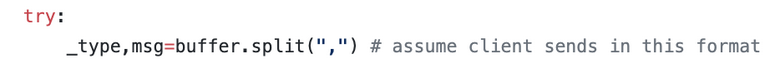
\includegraphics[width=\textwidth]{Assets/try.png}
\end{figure}

In the event that the server does not timeout, we will try to interpret the messages sent from the client. We assume the format of the client message is the type of message, followed by a comma, and followed by the content of the message. If the type of message is start, we create a new client object for the client and add it to our shared data structure. If the type is hwstart, we set up the global variable associated with the hardware token. if type is close, we do clean up for the client. It is important that information is kept in the shared structure so that client can reconnect later. If type of message is position, we will document row and column information for the client in our shared data structure across threads.
\section{Communications (Patrick)}

Our initial consideration is Wifi. It's very easy to work within our framework and we can easily setup connections for all clients to the other server. The usage of Wifi is also preferable given the Raspberry Pis have Wifi cards built in and can even be configured as an access point so this saves somewhat on cost. The specified range for Wifi for our Raspberry Pi Zero W is up to 100m although it should be expected that the range indoors will be much lower. This can be remedied with the purchase of an external antenna but we'll ideally only need 1 for the designated access point. The con here is that we'll have a single access point and many clients all within close proximity to one another, which will lead to significant signal interference. How much is yet to be seen but without knowing more about the conditions, it's hard to say if it'll be a significant problem.

    Bluetooth is also considered. Bluetooth transfers over the same frequency band as Wifi. Its strength mainly lies in communication between two points, with expansion up to 7 clients in a master-slave setup. By having a system like these, all the devices are automatically synced to the master's clock, which is very useful. However we desire a system that will be communicating with many clients so while it will work for a simple prototype, there would be no way to scale up using Bluetooth. Additionally the Raspberry Pi doesn't natively support a Bluetooth communication so a shield for the Pi would be necessary, incurring an additional cost. Finally the range matter of  In the end, it's determined that the strengths of Bluetooth don't fully align with our goals for this system.

    Zigbee is a radio based communication protocol based on the IEEE 802.15.4 specification. It has an upper limit of 100m line-of-sight. Zigbees can be attached to each Raspberry Pi and they would communicate . Their rated over-the-air communication link is 250MB/s which is more than enough for the small data packets that we're planning on sending over our network as detailed in our server-client descriptions. Zigbees have low power consumption, which aids in the long runtime that we're planning on having over the course of the ceremony. The Zigbee architecture requires 3 components - a coordinator, a router and the end devices. This would require extra hardware as these coordinator nodes are separate large components which likely won't last long on a battery pack. Zigbee, if the Wifi signal interference proves to be too great, would be our backup communication protocol.

In the end, Wifi was chosen as our desired communication protocol. Wifi was chosen for two main reasons: ease of use and cost effectiveness. To use something like Zigbee would require refitting all the Raspberry Pis with new receiver hardware whereas each Pi already comes pre-equipped with a Wifi chip. Also the ease of using Wifi with the Python framework makes it very attractive for getting a quick prototype up and running. Using TCP/IP we set up a socket based communication between the clients and the server. The clients have no need to communicate between each other, instead placing all the processing load on the server. This decision motivated the need for a better server processing unit. Perhaps if seeking pure robustness in our system and we had ample amounts of time, we would've opted for a Zigbee based network but Wifi has proven to be robust enough for our application that we're experiencing any detriment in performance.

\section{Hardware Token (Joey)}
\begin{figure}[H]
  \centering
      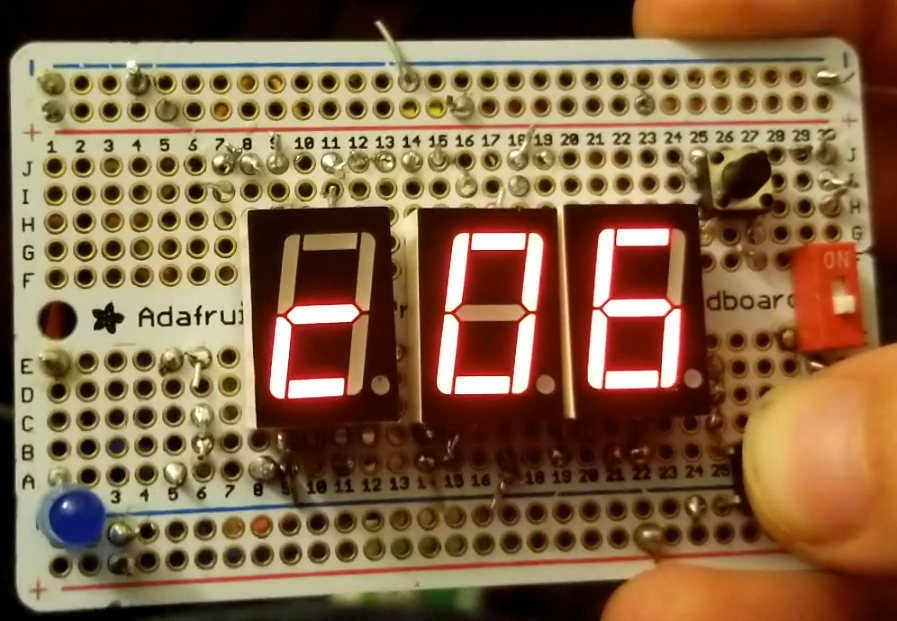
\includegraphics[width=0.8\textwidth]{Assets/input.png}
  \caption{Example of hardware token feedback for inputs. This shows that the user is currently at column 6. By flipping the switch on the right it will swap to displaying the current row position.}
\end{figure}

The Hardware token itself is a self contained device that allows for both inputs from the user regarding position information and feedback to the user about system status. It will display if it is connecting to the server, if it has successfully added the user as well as the currently inputted row and column number. The seven segment display is capable of outputting messages that will scroll across the screen. One example is when the token is attempting to connect to the server it will display "connecting" across the display.



\pagebreak
\begin{figure}[H]

  \centering

  \begin{tabular}{cc}

    % Requires \usepackage{graphicx}

    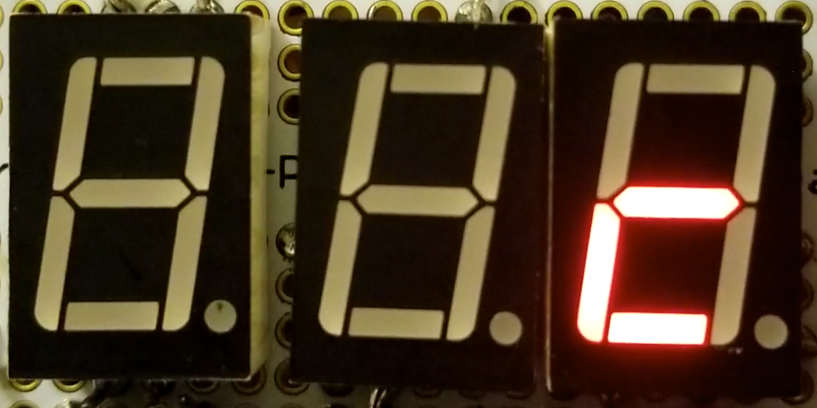
\includegraphics[width=60mm]{Assets/c.png}&

    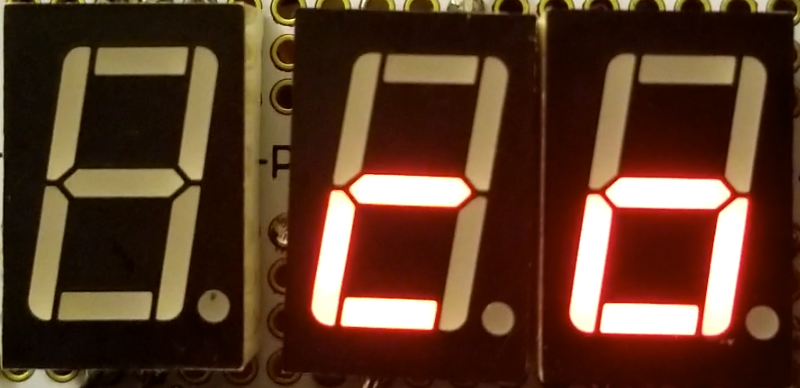
\includegraphics[width=60mm]{Assets/co.png}\\

    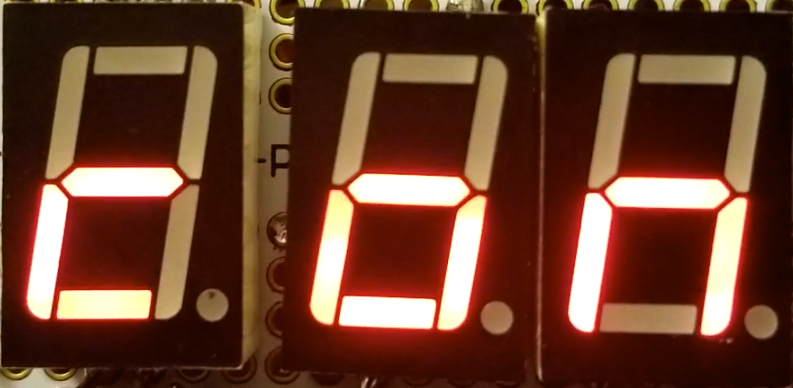
\includegraphics[width=60mm]{Assets/conn.png}&

    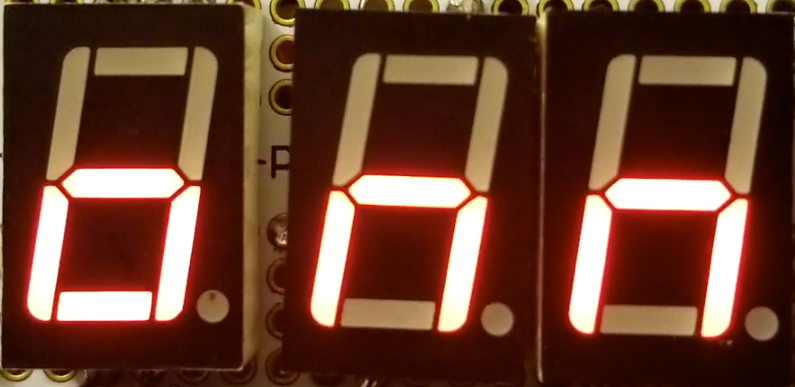
\includegraphics[width=60mm]{Assets/onn.png}\\

    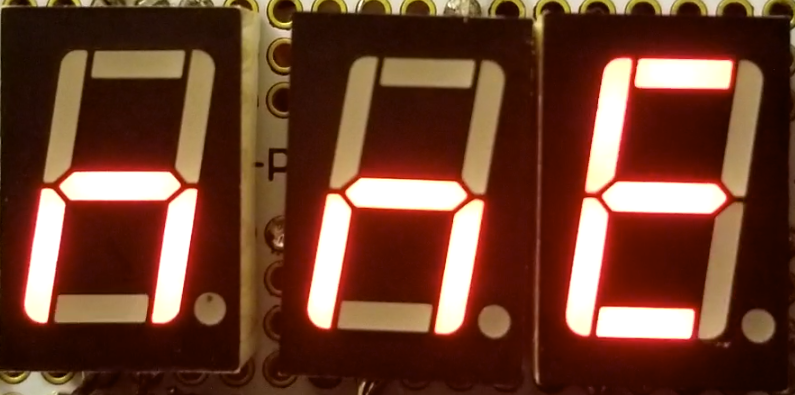
\includegraphics[width=60mm]{Assets/nne.png}&

    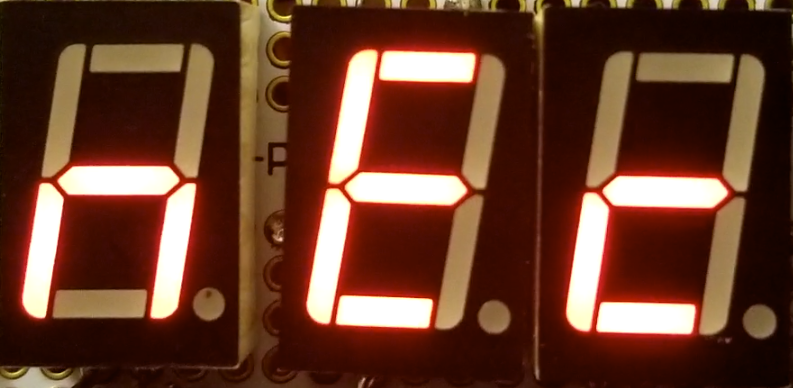
\includegraphics[width=60mm]{Assets/nec.png}\\
    
    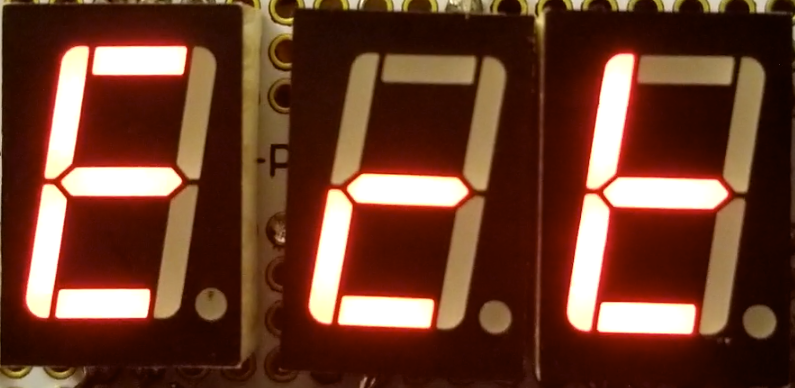
\includegraphics[width=60mm]{Assets/ect.png}&

    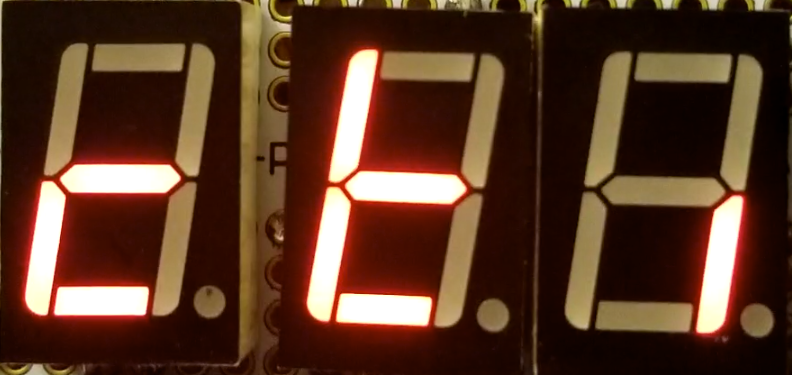
\includegraphics[width=60mm]{Assets/cti.png}\\
    
    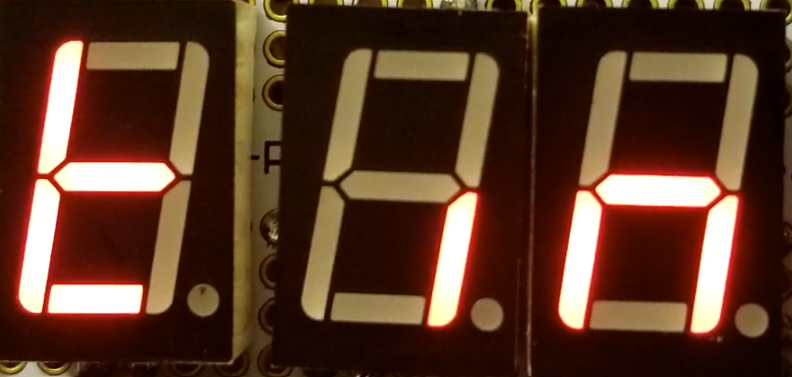
\includegraphics[width=60mm]{Assets/tin.png}&

    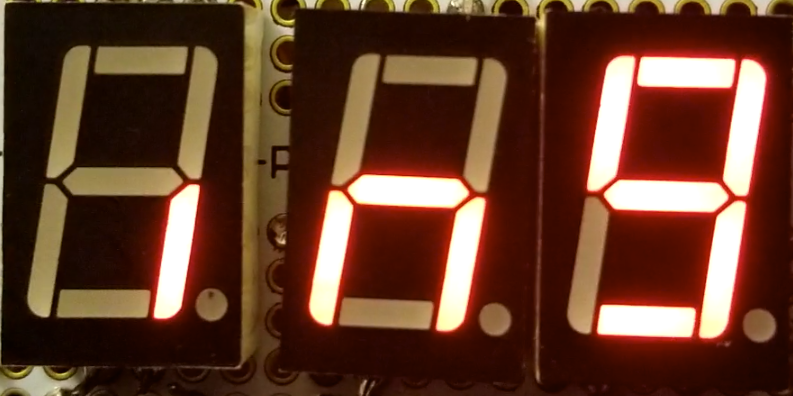
\includegraphics[width=60mm]{Assets/ing.png}\\
    
    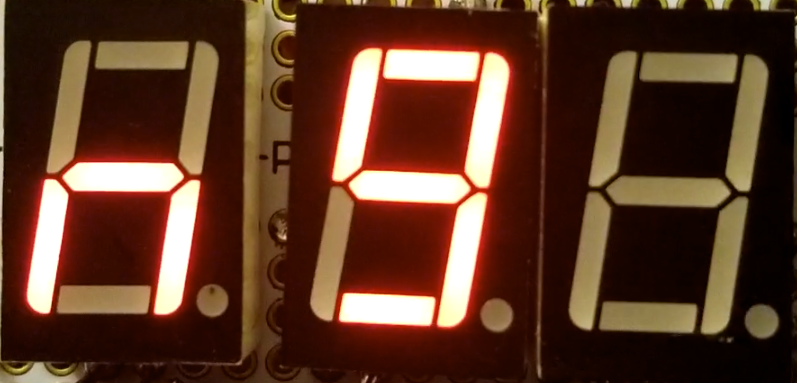
\includegraphics[width=60mm]{Assets/ng.png}&

    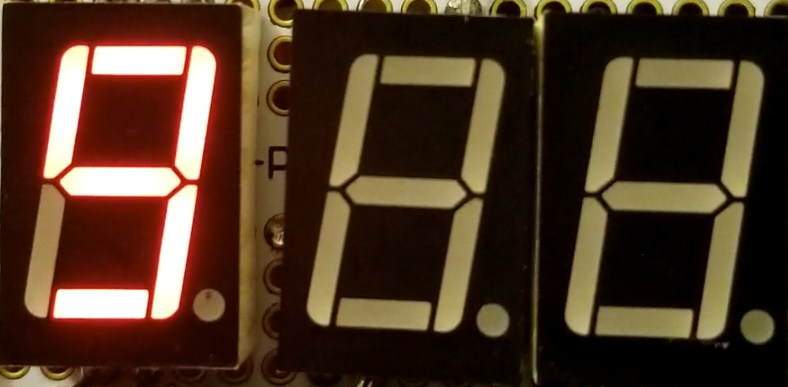
\includegraphics[width=60mm]{Assets/g.png}\\

  \end{tabular}
  
  \label{figur}\caption{When read left to right top to bottom, these are the individual frames for the word connecting being displayed across the 7 -segment display.}

\end{figure}

\pagebreak

\subsection{Hardware}
The hardware token, as the name implies, is made from hardware. The following parts list and wiring diagram explains how the system can be built in the event that one wishes to use one. In terms of circuit design, there are common cathode 7-segment displays that are connected to a current limiting resistor and the GPIO pins on the Raspberry Pi Zero W. There are also two capacitive debouncing circuits to allow for smooth voltage transitions on the button presses preventing multiple inputs from a single press. Finally there is an LED connected directly to a GPIO pin to a current limiting resistor and ground. This LED was originally to be used for indicating if the system has successfully added a user, but currently that role is taken by the displaying the string "success" across the 7-segment display. The LED will likely instead be used as a way to signal if the token's position info has been modified since the system added a prior user. If no use is found it will be removed from the final design.

\subsubsection{Parts List}
If one wishes to obtain the parts to purchase and assemble their own hardware token the following list can be used.
\begin{itemize}
\item 1 x Raspberry Pi Zero W
\item 3 x Common Cathode 7 segment displays
\item 2 x 1$\mu$F capacitors
\item 2 x Push Buttons
\item 1 LED
\item 1 x Toggle Switch
\item 5 x 1k$\Omega$ Resistors and 3 x 10k$\Omega$ Resistors
\end{itemize}

\subsubsection{Circuit Schematic}

\begin{figure}[H]
  \centering
      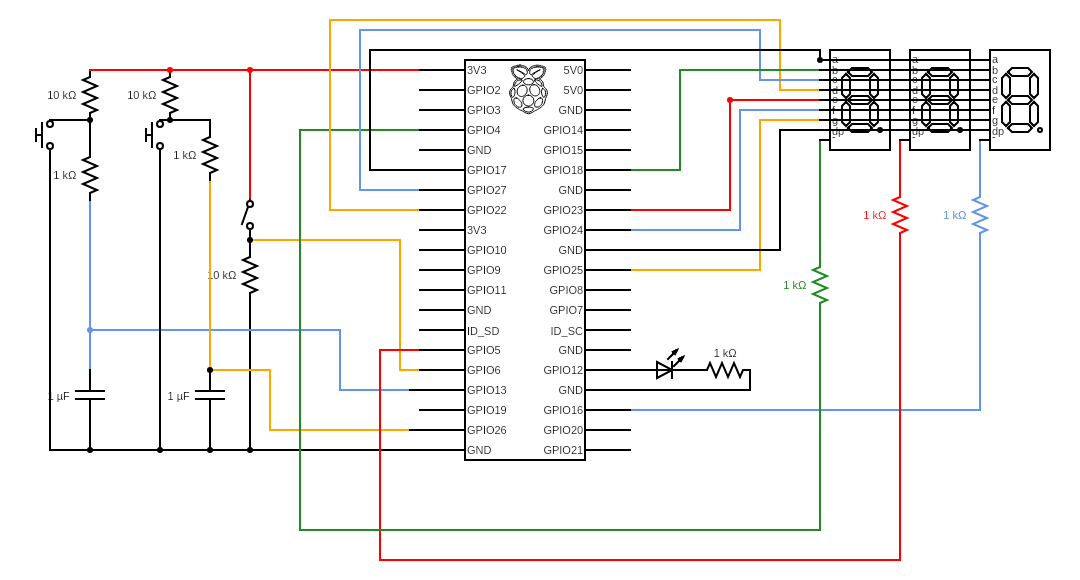
\includegraphics[width=0.95\textwidth]{Assets/circuit.png}
  \caption{Circuit schematic used for wiring the hardware token.}
\end{figure}

\subsection{Code}
The hardware token was written in C and has it's own makefile to allow for ease in compilation. It is made up of a total of 8 files in addition to the makefile: hardware.c, hardware.h, globals.h, hardware\textunderscore token.c, network.c, network.h, signal\textunderscore handler.c, and signal\textunderscore handler.h. The header files contain function declarations and global variables. All function declarations are commented to show what inputs/outputs are involved in the function as well as what the function is supposed to do.

\begin{figure}[H]
  \centering
      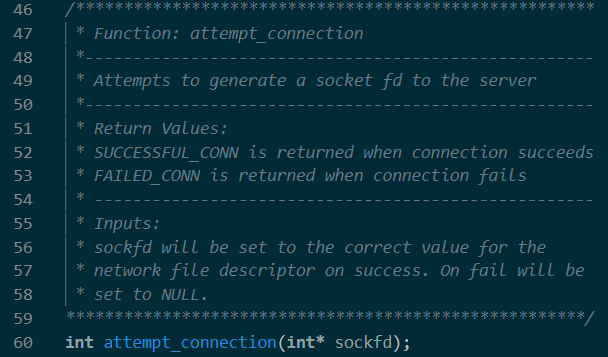
\includegraphics[width=\textwidth]{Assets/Comments.png}
  \caption{Example of comment info above function declarations. This is an example for what the attempt\textunderscore connection function in networks.h does.}
\end{figure}

All POSIX complient function calls that are made have proper error handling associated with them to ensure that the proper error code corresponding to errorno is printed to STDERR along with a message describing what went wrong. 

\begin{figure}[H]
  \centering
      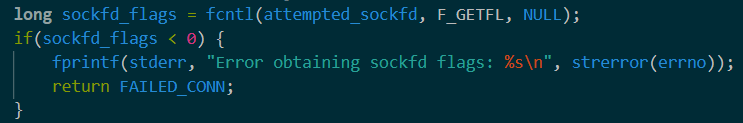
\includegraphics[width=\textwidth]{Assets/fcntl.png}
  \caption{Code showing error handling on POSIX function calls.}
\end{figure}

\subsubsection{Makefile}
\begin{figure}[H]
  \centering
      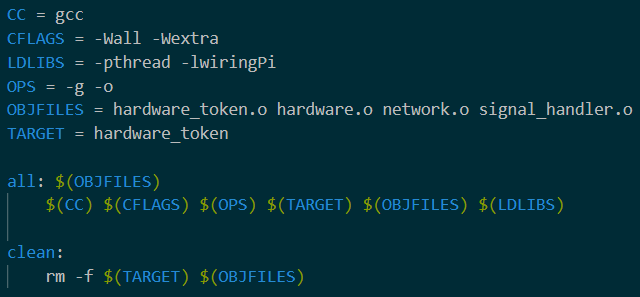
\includegraphics[width=0.8\textwidth]{Assets/Makefile.png}
  \caption{Code describing the Makefile.}
\end{figure}

The Makefile allows for an easy way to continue adding new files to the project and facilitate cleanup and compilation. It supports a make all option that makes the whole project and a clean option that deletes the object files produced.

\subsubsection{Globals.h}
This file contains globals that aren't unique to a type of file. These include delay paramaters that multiple functions use as well as modifiable global variables. The modifiable globals include a pthread mutex for concurrency related problems, row and column paramaters, messages to display on the segments and booleans used to determine when the program has finished, if the server is connected and whether or not there is a message to display.
\begin{figure}[H]
  \centering
      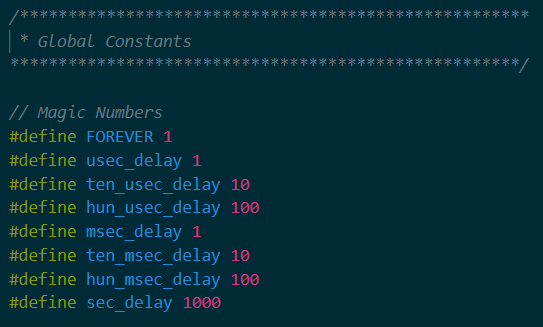
\includegraphics[width=0.75\textwidth]{Assets/global_constants.png}
  \caption{Code describing the Makefile.}
\end{figure}

\begin{figure}[H]
  \centering
      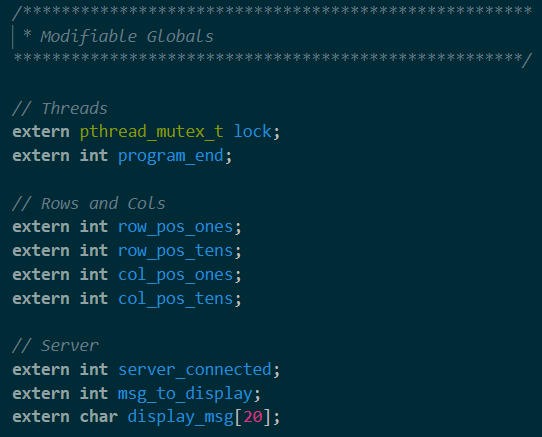
\includegraphics[width=0.75\textwidth]{Assets/modifiable_globals.png}
  \caption{Code describing the Makefile.}
\end{figure}

\subsubsection{Hardware Token.c}
This is the main file for the project that ties everything together. In here both of the pthreads are generated and used to start displaying information on the hardware token's display and begin communication with the server. 

\begin{figure}[H]
  \centering
      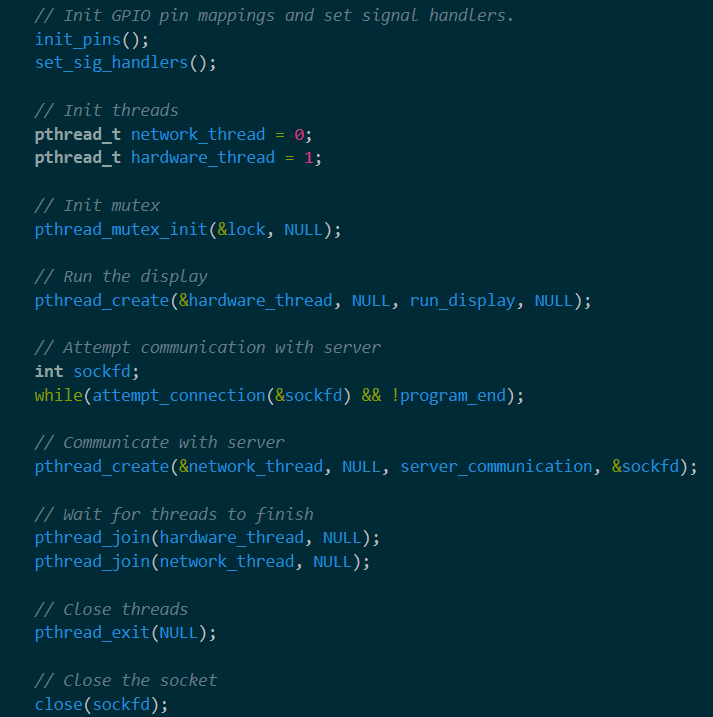
\includegraphics[width=0.75\textwidth]{Assets/hardware_token.png}
  \caption{Code describing the Makefile.}
\end{figure}

\subsubsection{Hardware.c and .h}
These files contain the global constants and functions needed to control the GPIO pins corresponding to physical hardware on the Pi. For brevity code snippets will be kept short in this section and will be used sparingly to show more complex implementations of certain functions. 

Two easy to get out of the way functions in this file include init\textunderscore pins and clear\textunderscore pins. These two do as one would expect and set the wiringPi GPIO pins to their proper start states and clear them all to zero respectively.

The real meat of this file includes the hardware thread function run\textunderscore display. This function runs while the program hasn't been set to the exit state by the signal handler. Once it is set to exit this thread and the network thread return and all data is properly cleaned up in the main function. If the hardware token is not connected to the server, it will continue to call the display\textunderscore connecting function that causes the 7 segment display to scroll the string "connecting" across its screen. If the hardware token is connected to the server it instead runs in the main display loop. It first checks if any message is ready to display and displays it if there is. It then reads inputs from the GPIO pins connected to the buttons. If the switch is set to rows then the code for button presses will modify the row variables and if it is set to cols then the column variables will be modified. It simply runs checks to make sure the 1's place overflows at 9 to 0 and 0 underflows to 9. when an underflow occurs the 10's place is modified so that it increments or decrements with similar under/overflow logic. Once this section completes it is time to blink the display. the blink\textunderscore segment function is called translating the integers to 7 segment bitmaps via the integer\textunderscore to\textunderscore display function and either 'r' or 'c' to the bitmap through the character\textunderscore to\textunderscore display function.

\begin{figure}[H]
  \centering
      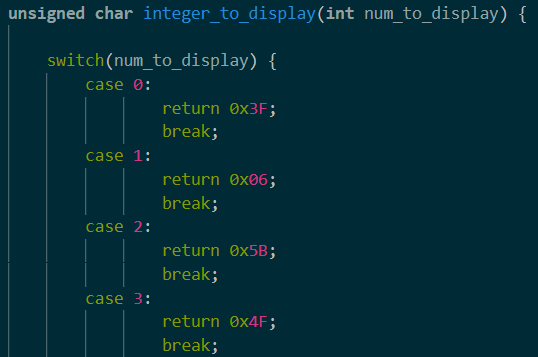
\includegraphics[width=\textwidth]{Assets/int_to_display.png}
  \caption{How integers are converted to 7 deg display outputs}
\end{figure}

\begin{figure}[H]
  \centering
      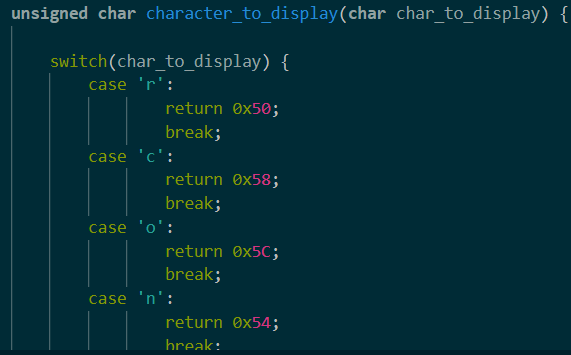
\includegraphics[width=\textwidth]{Assets/char_to_display.png}
  \caption{How  characters are converted to 7 deg display outputs}
\end{figure}

\begin{figure}[H]
  \centering
      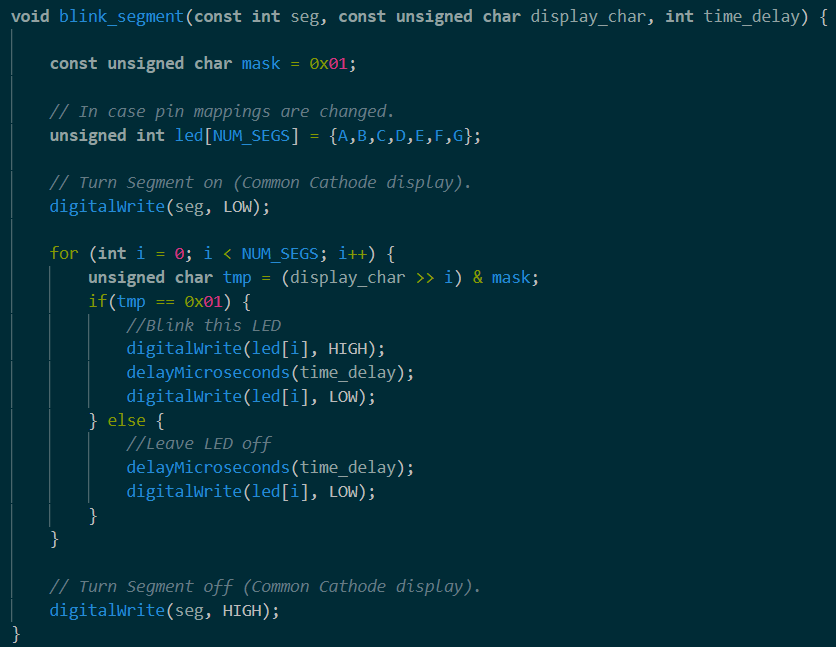
\includegraphics[width=\textwidth]{Assets/blink_segment.png}
  \caption{A mask is used to determine if the given segment is currently on or off. This is then used to blink the segment on for a small time then off again allowing the illusion of all displays being on at once.}
\end{figure}

The final function in these files worth noting is the display\textunderscore message function. This simply takes in some character array and blinks each segment through the blink\textunderscore segment function until it completes a full loop. While it is running no inputs from the buttons can affect the display since it would be problematic to have users affect the values they cannot see.

\subsubsection{Networks.c and .h}
As with the hardware code, code snippets will be used sparingly for brevity as the well over two thousand lines of code in these files would be a bit extensive to go over in great detail. These files have two functions. server\textunderscore communication and attempt\textunderscore connection. The first of the two is the function the network thread runs through and continues until the program ends. Similar to the hardware thread if a SIGINT or SIGTSTP occur the individual threads return and the program cleans up before exiting. The thread begins by running the following snippet to find the MAC Address of the token. Once it obtains it, it formats a message to deliver to the server:

 \begin{figure}[H]
  \centering
      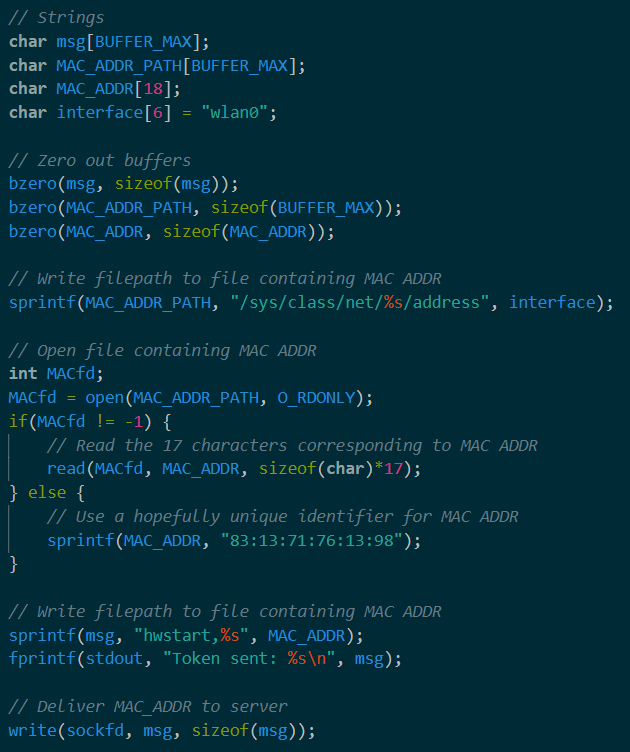
\includegraphics[width=0.85\textwidth]{Assets/MAC_ADDR_C.png}
  \caption{Code that obtains MAC ADDR. The comments sum up how it works.}
\end{figure}

It then while the server is connected will continue to read data from the server and send it current position and column data to keep the connection alive. Once it receives a message back from the server indicating someone has been added, it signals to the hardware thread that it is time to display "success" on the seven segment display. If the token is not connected to the server, it calls attempt\textunderscore connection.

While the server is attempting to connect to the server, it continues until the program ends to first generate a socket to the server using its IP address, set the socket to nonblocking and use connect in conjunction with select to obtain a timeout of exactly 2 seconds before reattempting communication. This allows for speedy program closes and reconnections if the server ever crashes. The default timeout on connect is way to long to allow for a speedy system. Once the server properly connects, the socket is set to blocking once again and the function returns SUCCESSFUL\textunderscore CONN (A 1 in the code).

\subsubsection{Signal Handler.c and .h}
These files handle the signal handling needed for the hardware token to work properly without crashing. The need for these functions is mostly due to the SIGPIPE signal. When the TCP socket connecting the token and the server is severed, a SIGPIPE is delivered from the OS to the program and if it isn't handled, the program is immediately stopped. Whenever the SIGPIPE comes through, the signal handler sets a global variable signaling to the hardware and network threads that the token is no longer connected. This causes connecting to display on the token while the network thread gets to work generating a new socket to attempt reconnection. SIGTSTP and SIGINT are two other signals handled by the signal handler. These are important for the program to properly exit while testing. This allows for all LEDs to properly shut off and network communication to successfully close out.

 \begin{figure}[H]
  \centering
      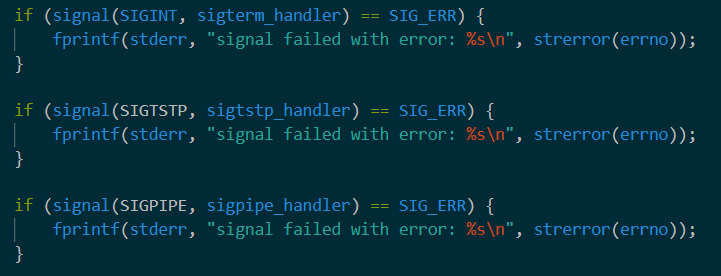
\includegraphics[width=\textwidth]{Assets/handlers.png}
  \caption{Code used to set signal handlers for various signals.}
\end{figure}

\subsection{Future Plans}
The hardware token is still not 100\% complete. There are a few small touches that will make the token more presentable, intuitive and robust. 

\subsubsection{3D Printed Case}
A 3D printed case will allow for printed instructions to remind users how to use the system as well as make the increment and decrement buttons more clear to the user. It also allows all the internals to be hidden away from the user and provides padding in case the device is dropped during the graduation ceremony. It also allows for the token to have a more aesthetically pleasing design giving it a much more professional look and feel.

\subsubsection{PCB}
\begin{figure}[H]
  \centering
      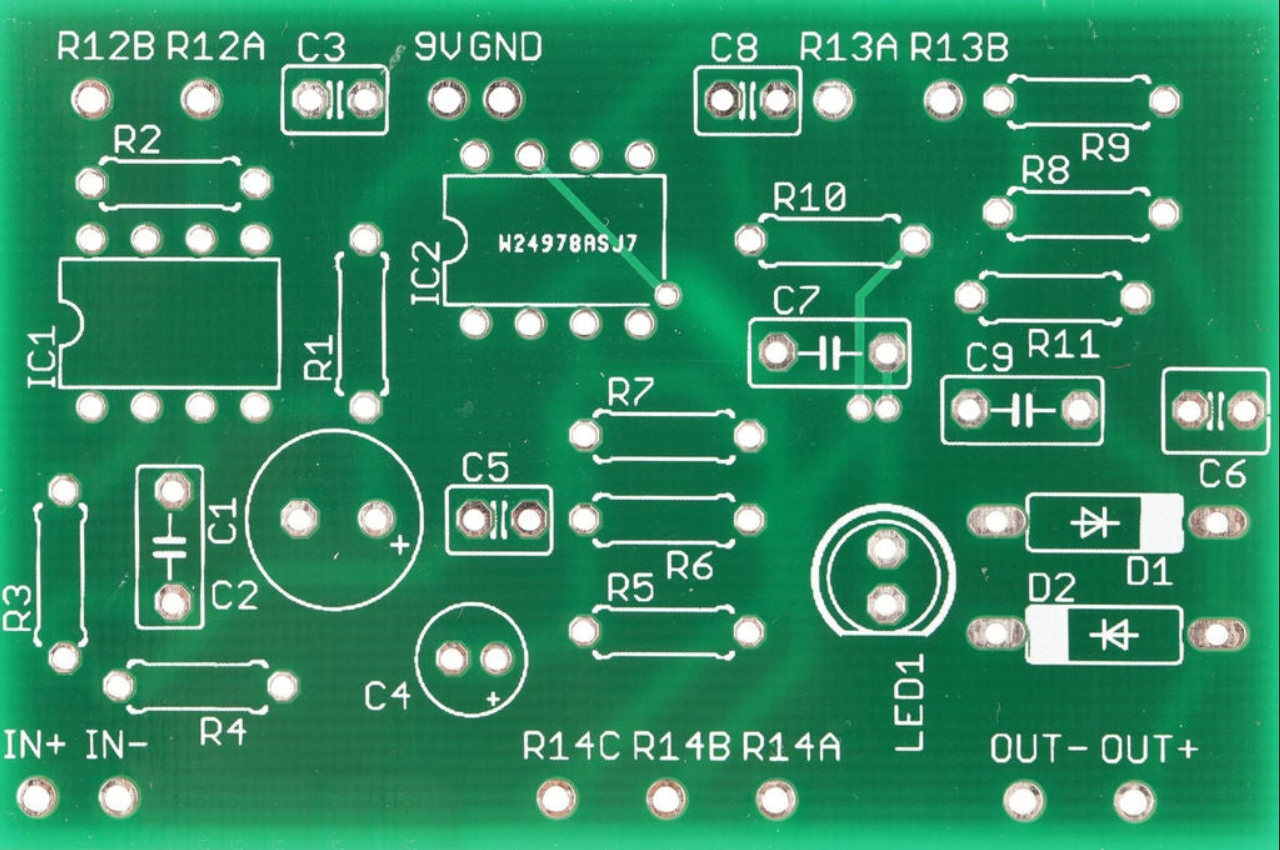
\includegraphics[width=0.5\textwidth]{Assets/PCB.png}
  \caption{Sample printed circuit board that shows how easily components could be soldered together without worrying about cutting and soldering connecting wires.}
\end{figure}

Having a printed circuit board for soldering the components for the hardware token will significantly reduce the difficulty in connecting all of the components together and allow for a more compact design. This will make development of a 3D printed case easier and allow for case designs to be more compact as well.

\subsubsection{Using RFID to Initialize Position Data}
\begin{figure}[H]
  \centering
      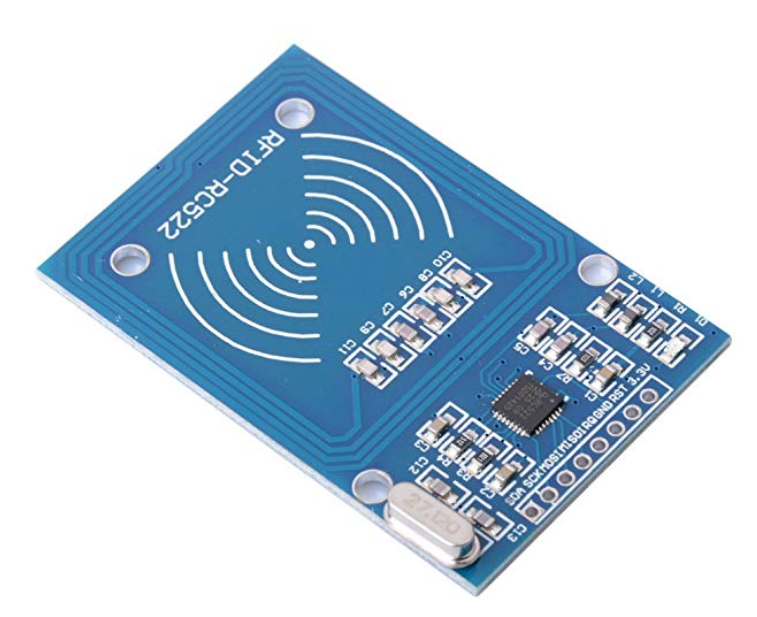
\includegraphics[width=0.5\textwidth]{Assets/RFID.png}
  \caption{RFID reader that is currently planned to be integrated as a means of connecting oneself to the server.}
\end{figure}

Currently the system supports having each individual cap having a button that will be pressed when someone wishes to tell the server to poll the hardware token and input their position into the system. This leads to a few issues involving people accidentally inputting themselves into the system when they don't have the hardware token. These issues can easily be circumvented by use of RFID integrated into the client caps that reads from the hardware token to decide whether to transmit or not. Since RFID is only accurate up to a few centimeters, there would be no way to false input oneself into the system. All that would be required from a user would be to pull the hardware token up to the graduation cap to send one's current position to the server. RFID can be obtained very cheaply on Amazon, a pack of 5 readers and tokens run for a little over \$10. 

\section{Conclusion}
\begin{figure}[H]
  \centering
      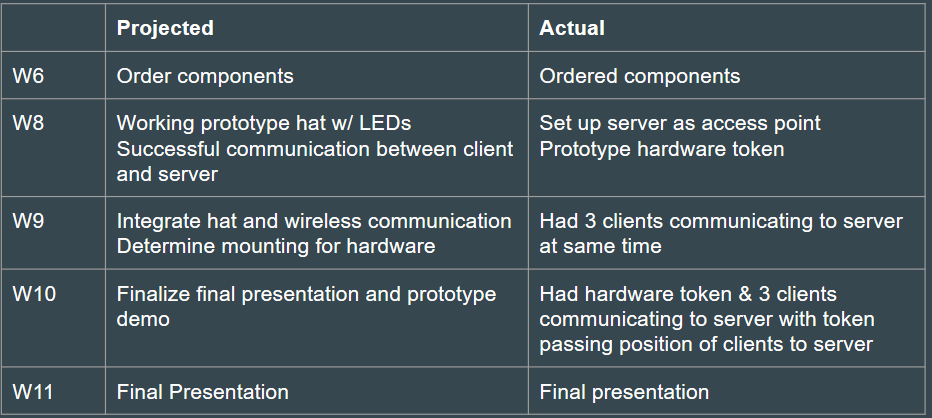
\includegraphics[width=\textwidth]{Assets/Timeline.png}
  \caption{Chart of the expected vs. actual timeline we followed this quarter.}
\end{figure}
Overall the project this quarter has gone successfully this quarter. While we were unable to meet our original timeline exactly, despite the complications, we managed to follow it pretty closely and adapted our goals according to the setbacks that arose (mostly related to the lack of hardware for the caps). This allowed us to continue moving forward throughout the quarter and ensured everyone always had something to work on. Despite the setbacks we faced throughout the quarter we managed to adhere closely to our initial timeline. Although a challenging project, we were able to divide the work equally amongst our group. We have learned to work as an effective unit, not afraid to ask one another for help when we need it.

\end{document}

